% vim: set tw=78 tabstop=4 shiftwidth=4 aw ai:

\chapter{Deploying Peer-to-Peer Network Infrastructures through
Virtualization}
\label{chapter:virt-infra}

With respect to network protocol and applications, two kinds of environments
are generally used for testing, measurements, evaluation and analysis: lab
setups and real world experiments. Lab setups or experimental setups are
custom setups for protocol evaluation; the experimenter has full control of
the environment. This is typically the case for functionality testing or
experiments in which the experimenter needs full control of the process. The
experimenter may use a lab-based infrastructure, a cluster/cloud based one, or
one provided by the community, such as
PlanetLab\footnote{\url{http://www.planet-lab.org/}}. Rias~\cite{rias} is an
example of an overlay topology created on top of a PlanetLab infrastructure.

\section{Virtualization Solutions}
\label{sec:virt-infra:openvz}

An important ``buzzword'' in the last decade, virtualization technology has
broken ground from its theoretical base in the late 70s to a diversity of
full-fledged implementations nowadays. With the continuous increasing capacity
of HDD space, memory and CPU power (mostly in number of cores), virtualization
solutions provide the best way for proper allocation of resources. New
features such as hardware-assisted virtualization, I/O improvements, live
migration have ignited the demand for efficient virtualization solutions that
consolidate current and future hardware resources.

\subsection{Benefits of Virtualization}

Virtualization solutions have made their way in day-to-day uses as they
provide important benefits, especially regarding costs. A specific hardware
system may be able to run different instances of operating systems, while, in
the absence of virtualization, more systems would be required.

Three important benefits have been identified~\cite{best-damn-virt} for
virtualization:

\begin{itemize}
  \item consolidation;
  \item reliability;
  \item security.
\end{itemize}

\textbf{Consolidation}, a particularly important aspect in the business world,
allows the ``unification'' of resources on top of a few physical platforms. The
ever increasing CPU power, I/O speed and memory capacity may now be used to
provide sufficient resources for multiple virtualized operating systems.
Modern data centers must be plugged even when nothing is really running,
resulting in infrastructure waste. The use of virtualization solutions and
migration techniques allows the unification of multiple virtual servers on
shared hardware.

Virtualization solutions provide \textbf{reliability} through isolation. A
failure on a given virtual machine will not affect another virtual machine.
The ``partitioning'' employed by a virtualization solution means that each
virtual machine is running on a dedicated specialized simulated hardware. The
isolation and partitioning allow dynamic allocation of new systems whenever
required without the need to acquire additional hardware.

Isolation provided by virtualization technology is a key feature for ensuring
security of virtual machines. If a given virtual machine faults or has been
compromised, it does not affect other systems and, in need, it may be rapidly
disabled. This would be very difficult to achieve on a physical
infrastructure.

\subsection{OpenVZ}

As OS-level virtualization had proven to be the way to go for building up a
Peer-to-Peer infrastructure, we had to chose between existing solutions such
as OpenVZ, LXC, V-Server. As we have good experience with Linux, the solution
had to be a Linux-based solution. We had to chose between OpenVZ, LXC,
V-Server. Though LXC currently possesses the advantage of being active in the
mainline kernel, it was still in its infancy in the time we started building
the infrastructure. Apart from that, documentation is quite scarce. Between
OpenVZ and V-Server, we chose OpenVZ due to its high quality documentation
and peer recommendation and experience.

Just as other OS-level virtualization solutions, OpenVZ is a series of patches
to the Linux kernel that enhances process and resource isolation among
containers. Major Linux distributions typically ship an OpenVZ able kernel that
is easily installable. A series of user space tools allow installation and
configuration of virtual machines. Typically, most commands and keywords start
with the \texttt{vz} prefix.

As an OS-level solution, with easy network configuration and a flexible
resource limit configuration interface, OpenVZ was considered to be the most
suitable solution for deploying a virtualized network infrastructure. The
later chapters will provide insight on the process and tools employed for
creating the infrastructure and deploying Peer-to-Peer swarm scenarios.

\section{Virtualized Peer-to-Peer Infrastructure Setup}
\label{sec:virt-infra:setup}

Creating a virtualized environment requires the hardware nodes where virtual
machines will be deployed, the network infrastructure, a set of OpenVZ
templates for installation and a framework that enables commanding clients
inside the virtual machines.  Each virtual machine runs a single BitTorrent
application that has been instrumented to use an easily-automated CLI.

Despite its limitations, OpenVZ is the best choice for creating a virtualized
environment for evaluating BitTorrent clients. Its minimal overhead and
low-resource consumption enables running tens of virtual machines on the same
hardware node with little penalty.

\subsection{Overall View}
\label{sec:virt-overall}

%The above mentioned values assume the usage of the hrktorrent/libtorrent
%BitTorrent client. They also assume the scheduling impact of all processes in
%the VEs induces low overhead on the overall performance. However, even
%considering the scheduling overhead, a modest system would still be able to
%run at least 10 to 20 VEs.

% TODO: mention virtualization measurements

Through experimentation, we concluded that a virtualized testing environment
based on OpenVZ would provide similar testing capabilities as a
non-virtualized cluster with at most 10\% of the cost. Our  experimental setup
consisting of just 10 computers is able of running at least 100 virtualized
environment with minimal loss of performance.

\begin{figure}
  \begin{center}
    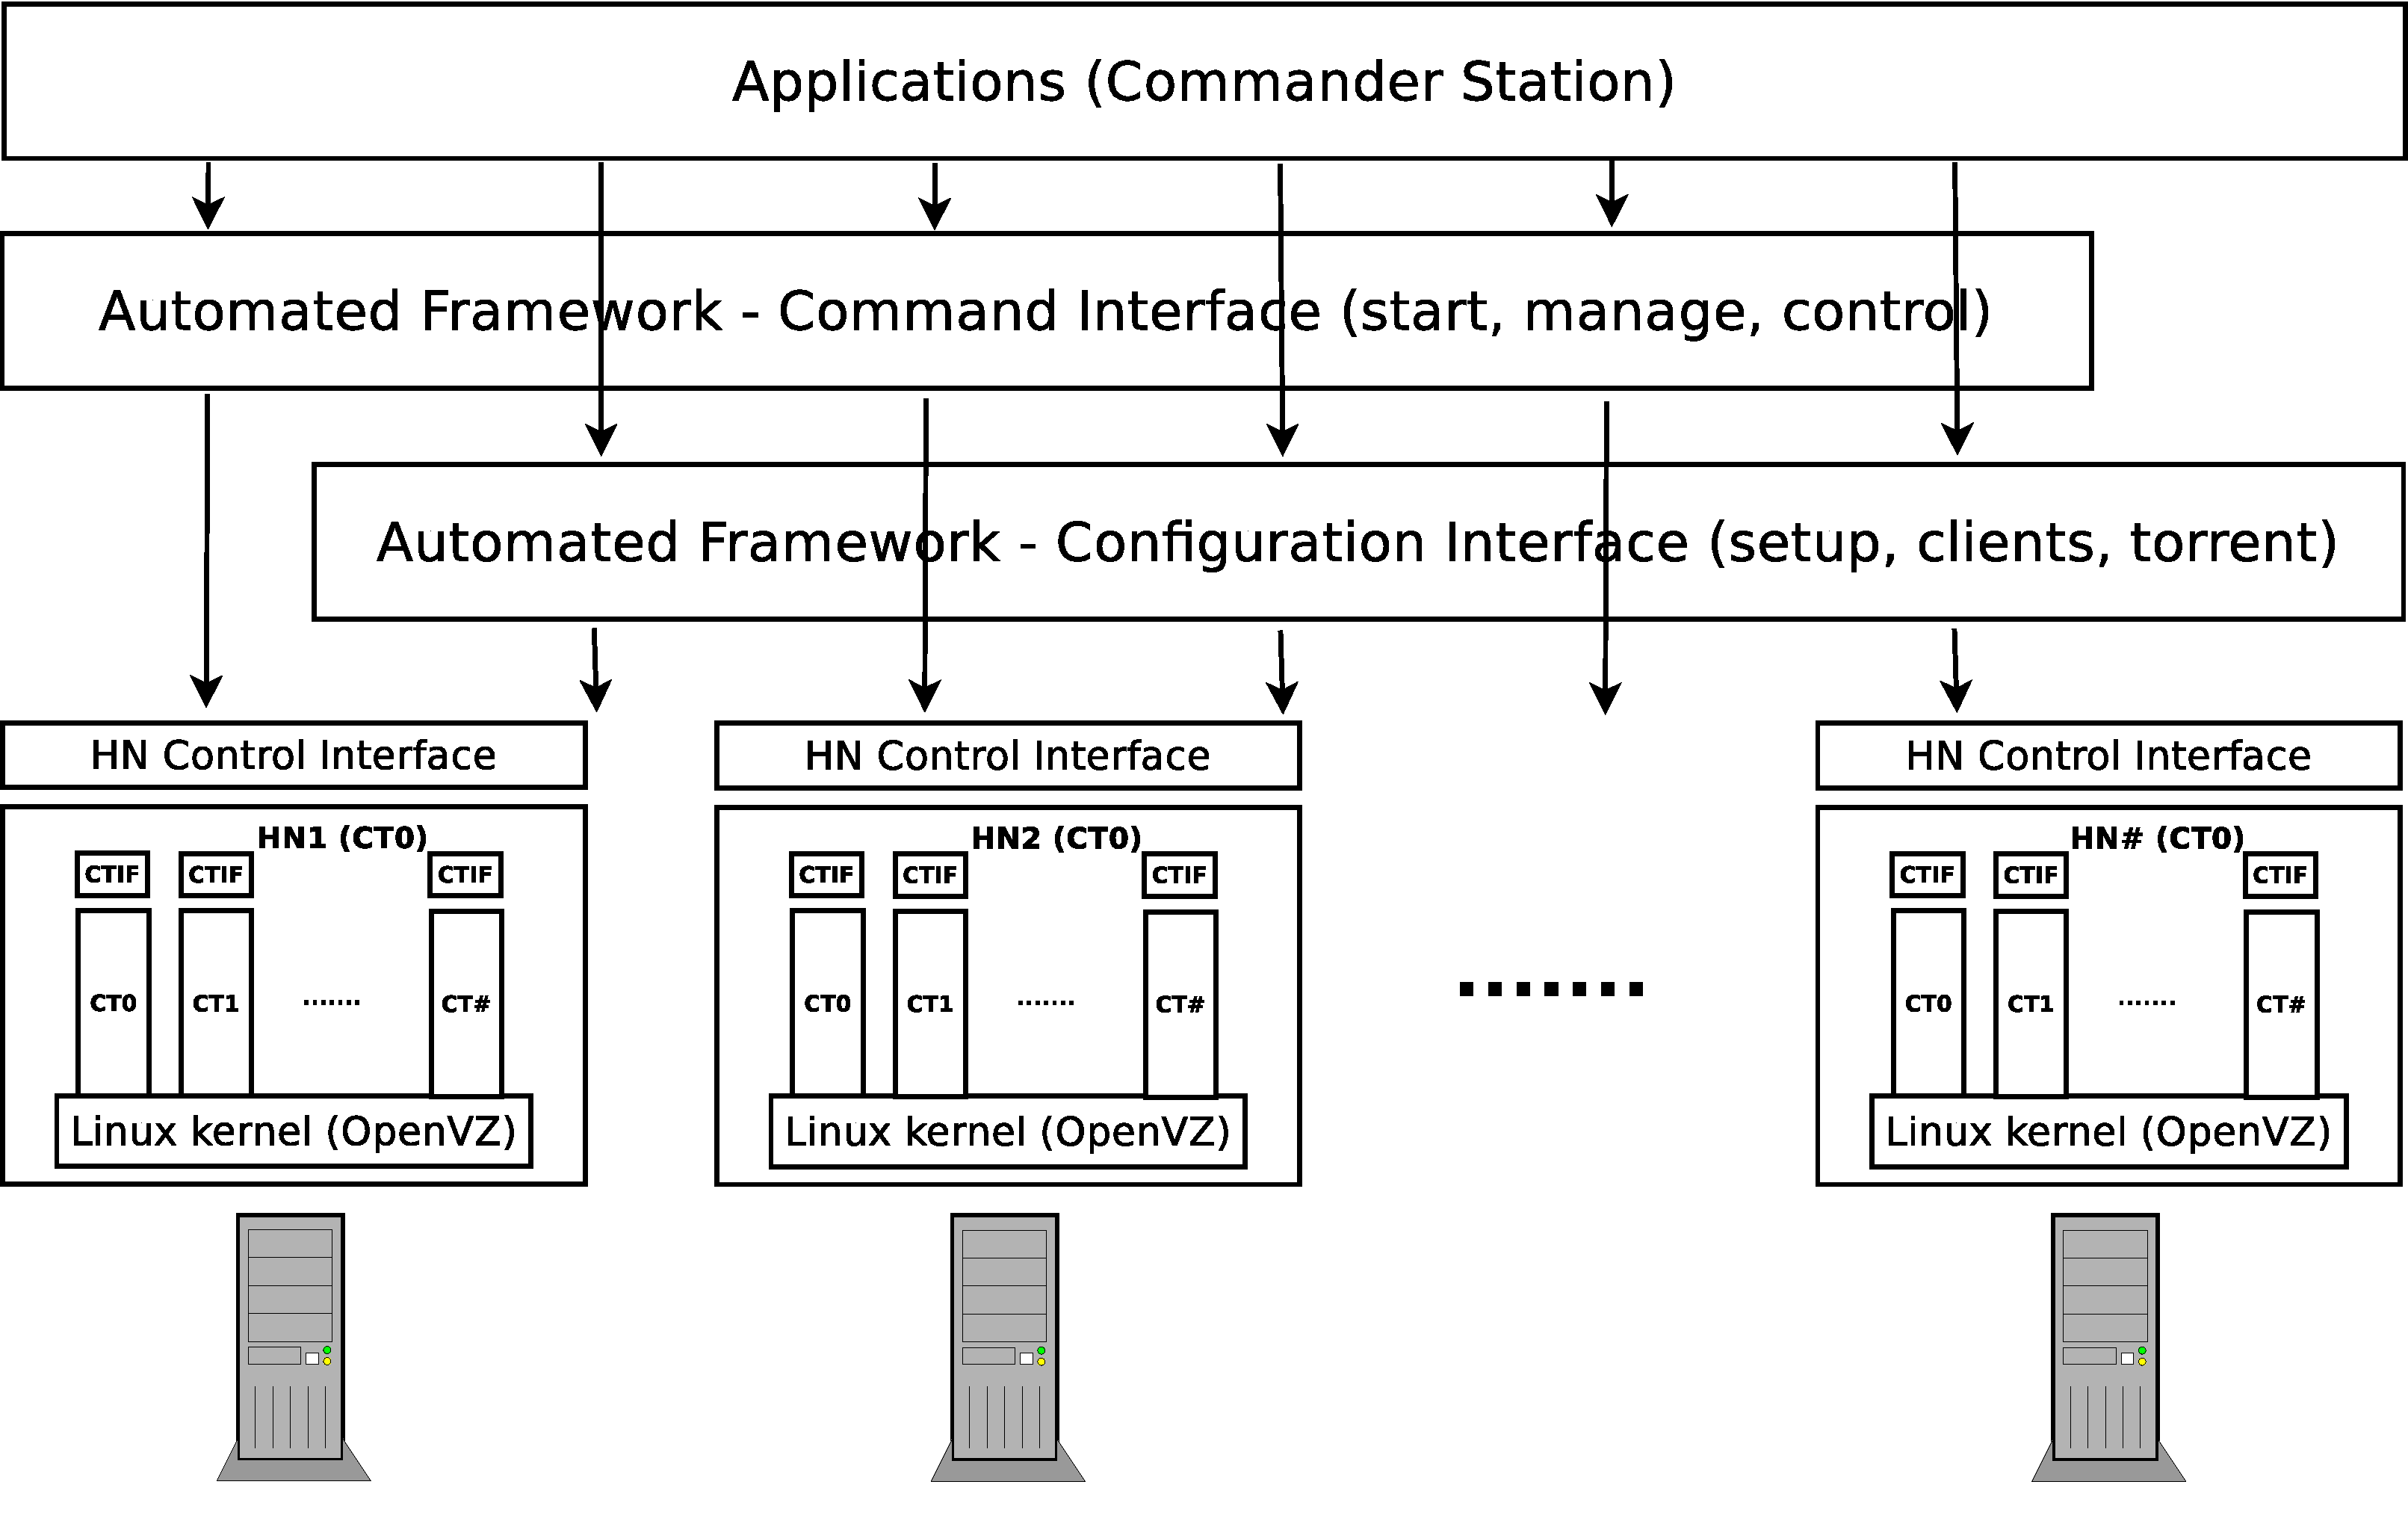
\includegraphics[width=0.7\textwidth]{src/img/virt-infra/virt-infra-overview}
  \end{center}
  \caption{Infrastructure Overview}
  \label{fig:virt-infra:infrastructure-overview}
\end{figure}

Figure~\ref{fig:virt-infra:infrastructure-overview} presents a general
overview of the BitTorrent Testing Infrastructure.

The infrastructure is design to run commodity hardware systems. Each system
uses OpenVZ virtual machine implementation to run multiple virtual systems on
the same hardware node.  Each virtual machine contains the basic tools for
running and compiling the BitTorrent clients. BitTorrent implementations have
been instrumented for automated command and also for outputting status and
logging information required for subsequent analysis and result
interpretation. As the infrastructure aims to be generic among different
implementation, the addition of a new BitTorrent client means adding the
required scripts and instrumentation.

The virtualized environment is thus a cheaper and more flexible alternative to
a full-fledged cluster with little performance loss. Its main disadvantage is
the asymmetry between virtualized environments that run on different hardware
system. The main issue is network bandwidth between VEs running on the same
hardware node and VEs running on different hardware nodes. This can be
corrected by using traffic limitation ensuring a complete network bandwidth
symmetry between the VEs.

\section{Evaluating Virtualization}

With a plethora of virtualization solutions, a infrastructure for deploying
Peer-to-Peer scenario has to take into account the adequacy of each solution.
Through empirical studies we have chosen OpenVZ as a suitable solution for our
needs, with the lack, however, of a formal evaluation method.

Considering the use of virtualization solutions for our purpose we consider
three important dimensions:

\begin{itemize}
  \item \textbf{efficiency} (scalability) -- how many virtual
  machines/containers may be deployed on a virtual host and allow proper
  simulation of an environment;
  \item \textbf{isolation} -- how well are virtual machines' resources
  separated;
  \item \textbf{reliability} -- how many software crashes happen for a given
  solution; this may be due to implementation or to resourse overuse/abuse.
\end{itemize}

Wood~et~al.~\cite{virt-prof-model} have investigated VMware ESX and Xen and
created an I/O model and profile.

An approach similar to ours was undertaken by
Soltesz~et~al.~\cite{virt-doppel}. They considered Xen and Linux Vservers as
the representatives for para- and paene-virtualization. Their metrics included
performance, isolation and scalability with similar meanings ar to ours.

\textbf{Efficiency} is a sheer measure of deploying large numbers of virtual
machines and containers on top of a given hardware system.
Padala~et~al.~\cite{eval-virt-performance} have shown that OpenVZ possesses a
smaller overhead compared to Xen. However, no formal method has been employed
and their study doesn't take into account other OS-level virtualization
solutions.

A formal measurement for virtualization efficiency/performance should consider
three aspects:

\begin{itemize}
  \item hardware resources;
  \item software implementation (in our case, BitTorrent client
  implementation);
  \item virtualization solution.
\end{itemize}

As such, we formalize efficiency as a function of the three dimensions above:

\begin{align}
Eff & = f(HW, SW, VS)\\
Eff & = f(RAM, HDD, CPU, NET, OS, PS, BT, VS, NVM)\\
Eff &= \frac{VMB}{HNB}
\end{align}

where:

\begin{multicols}{2}
    \begin{itemize}
      \item \texttt{Eff}: efficiency/performance
      \item \texttt{HW}: hardware resources
      \item \texttt{SW}: software implementation
      \item \texttt{VS}: virtualization solution
      \item \texttt{RAM}: system RAM
      \item \texttt{HDD}: I/O space
      \item \texttt{CPU}: processor power
      \item \texttt{NET}: networking features
      \item \texttt{OS}: operating system implementation
      \item \texttt{PS}: basic container processes
      \item \texttt{BT}: BitTorrent implementation
      \item \texttt{NVM}: number of virtual machines
      \item \texttt{VMB}: virtual machine behavior
      \item \texttt{HNB}: hardware node behavior
    \end{itemize}
\end{multicols}

\textbf{Isolation} is a means of stating how well is a virtual machine
separated from another virtual machine and from the base system. As OpenVZ VEs
are using the same kernel, it is obvious the isolation value is less than that
of Xen of KVM. Isolation serves as an important dimension for measuring
virtualization solution adequacy. The ability to completely isolate a virtual
machine and properly specify its resource usage allows better resemblance to a
base hardware system.

While we find it difficult to properly formalize isolation we consider
achievable a ``virtualization isolation scale'' in which virtualization
solutions may be compared against each other. A rather relative value than an
absolute one. Thus we consider it safe to state that:

\begin{align}
Iso(normal processes) < Iso(chroot) < Iso(OpenVZ, LXC) < Iso(Xen,KVM)
\end{align}

A careful analysis of virtualization solutions, facilities employed, how well
is separation achieved and resource limitation enforced must be undertaken. It
will allow proper relative scale placing of virtualization solutions.

\textbf{Reliability} must be considered when dealing with a heavily used
infrastructure when evaluating multiple virtualization solutions. In our
experience we have encountered several software problems such as disk
inconsistency, operating system level errors and lack of responsiveness due to
the high (ab)use of hardware resources. Our OpenVZ based infrastructure must
be evaluated. Fortunately, there are a number of well defined and thoroughly
analysed measures such as \textit{failure rate} of \textit{mean distance
between failures} that can be taken into account. These have to consider the
evaluating environment, as with the efficiency dimension:

\begin{align}
Rel & = f(HW, SW, VS)\\
Rel & = f(RAM, HDD, CPU, OS (filesystem), PS, BT, VS, NVM)
\end{align}

Properly defined and evaluated dimensions such as efficiency, isolation and
reliability provide an overall view of virtualization solutions and their
adequacy for our specific purpose. We consider there is no ``silver bullet''
solution but rather one that will provide suitable for a class of necessities.
The weight one maps to each of the dimensions would depend on his/her needs
and environment specifics.

More than this, it may not be feasible (nor possible) to extract a formula
taking into account all input data. Rather consider a numeric value for each
metric and ensure a comparison between these values. Such that one may
conclude that affecting one input variable into one direction (increase or
decrease) will have a certain impact on the metric. This is the similar
approach provided by Ismail~et~al.~\cite{virt-metrics}.

We have experimented both with OpenVZ, LXC and Xen-based environment in order
to create a proper experimental testbed for the above metrics.

In OpenVZ's case, our study focused on efficiency/scalability. Active VEs
running the hrktorrent client use about 70 to 170MB of RAM. This gives a rough
estimate of about $[20 MB; 40 MB]$ memory consumption per VE. The basic system
also uses at most 120MB of RAM.

Table~\ref{table:virt-infra:openvz} gives a low limit for the number of OpenVZ
virtual environments able to run on a basic PC. Italic means limitation is due
to RAM capacity, while bold means limitation is due to HDD space.

\begin{table}[ht]
  \centering
  \begin{tabular}{|r|r|r|r|r|r|}
    \hline
     & \multicolumn{5}{|c|}{\textbf{Memory}} \\
    \hline
    \textbf{HDD} & \textbf{1GB} & \textbf{2GB} & \textbf{4GB} & \textbf{8GB} &
    \textbf{16GB} \\
    \hline
    80GB & \textbf{7} & \textbf{7} & \textbf{7} & \textbf{7} &
    \textbf{7} \\
    \hline
    120GB & \textbf{12} & \textbf{12} & \textbf{12} & \textbf{12} &
    \textbf{12} \\
    \hline
    200GB & \textbf{22} & \textbf{22} & \textbf{22} & \textbf{22} &
    \textbf{22} \\
    \hline
    300GB & \textit{22} & \textbf{35} & \textbf{35} & \textbf{35} &
    \textbf{35} \\
    \hline
    500GB & \textit{22} & \textit{47} & \textbf{60} & \textbf{60} &
    \textbf{60} \\
    \hline
    750GB & \textit{22} & \textit{47} & \textbf{91} & \textbf{91} &
    \textbf{91} \\
    \hline
    1TB & \textit{22} & \textit{47} & \textit{97} & \textbf{122} &
    \textbf{122} \\
    \hline
  \end{tabular}
  \caption{Scalability in OpenVZ (Number of Containers)}
  \label{table:virt-infra:openvz}
\end{table}

In case of LXC, we've run a scenario involving the use of the Unix gzip
command, used for file compression. This allowed us to measure both CPU and
hard-disk related values concerned with scalability. Tables below present CPU
usage, I/O operations per second disk busy percentage.

\begin{table}[ht]
  \centering
  \begin{tabular}{@{}rrrrr@{}}
    \toprule
    \textbf{No. containers} & \textbf{Average} & \textbf{Maximum} &
    \textbf{Minimum} & \textbf{Time} \\
    & \textbf{(\%)} & \textbf{(\%)} & \textbf{(\%)} &\textbf{(s)} \\
    \midrule
    2 & 19.2 & 21.3 & 18.7 & 2626 \\
    4 & 39.0 & 44.0 & 35.4 & 2786 \\
    8 & 82.3 & 95.6 & 70.6 & 2401 \\
    \bottomrule
  \end{tabular}
  \caption{LXC CPU Usage for gzip}
  \label{table:virt-infra:lxc-cpu}
\end{table}

\begin{table}[ht]
  \centering
  \begin{tabular}{@{}rrrrr@{}}
    \toprule
    \textbf{No. containers} & \textbf{Average} & \textbf{Maximum} &
    \textbf{Minimum} & \textbf{Time} \\
    & \textbf{(ops/s)} & \textbf{(ops/s)} & \textbf{(ops/s)} &\textbf{(s)} \\
    \midrule
    2 & 41.5 & 104.4 & 17.0 & 2626 \\
    4 & 39.0 & 174.2 & 29.2 & 2786 \\
    8 & 176.6 & 275.4 & 84.6 & 2401 \\
    \bottomrule
  \end{tabular}
  \caption{LXC I/O operatinons for gzip}
  \label{table:virt-infra:lxc-io}
\end{table}

\begin{table}[ht]
  \centering
  \begin{tabular}{@{}rrrrr@{}}
    \toprule
    \textbf{No. containers} & \textbf{Average} & \textbf{Maximum} &
    \textbf{Minimum} & \textbf{Time} \\
    & \textbf{(\%)} & \textbf{(\%)} & \textbf{(\%)} &\textbf{(s)} \\
    \midrule
    2 & 11.8 & 32.3 & 5.3 & 2626 \\
    4 & 26.1 & 65.9 & 12.4 & 2786 \\
    8 & 61.3 & 85.4 & 36.2 & 2401 \\
    \bottomrule
  \end{tabular}
  \caption{LXC Disk Busy for gzip}
  \label{table:virt-infra:lxc-disk}
\end{table}

In case of Xen we've used four virtual machines, each using 256MB of RAM and
running on a single core of the base system. These virtual machines were
running ffmpeg, an application for video conversion. Results of CPU and disk
usage are presented in Table~\ref{table:virt-infra:xen-metrics}.

\begin{table}[ht]
  \centering
  \begin{tabular}{@{}lrrr@{}}
    \toprule
    \textbf{Metric} & \textbf{1 VM} & \textbf{2 VMs} & \textbf{3 VMs} \\
    \midrule
    CPU Usage (\%) & 18.49 & 22.07 & 26.85 \\
    Disk writes (bytes/s) & 1008.11 & 1820.96 & 5074.22 \\
    Running Time (s) & 483 & 908 & 1808 \\
    \bottomrule
  \end{tabular}
  \caption{Xen Metrics for ffmpeg}
  \label{table:virt-infra:xen-metrics}
\end{table}

The evolution of various metrics is slightly over-linear in case of disk usage
and close to linear in case of running time. Xen scaling is similar to LXC in
case of running resource intensive applications such as ffmpeg. However, each
virtual machine uses a predefined value for memory which is generally higher
than an operating system-level virtualization solution due to the new kernel
memory and hypervisor overhead.

\section{Automating Deployment and Management of Peer-to-Peer Clients}
\label{sec:virt-infra:auto-deploy}

On top of the virtualized infrastructure, we developed a framework for
running, commanding and managing BitTorrent swarms. The purpose is to have
access to an easy-to-use system for deploying simple to complex scenarios, make
extensive measurements and collect and analyze swarm information (such as
protocol messages, transfer speed, connected peers).

\textit{The swarm management framework}~\cite{swarm-management} is a service-based infrastructure that
allows easy configuration and commanding of BitTorrent clients on a variety of
systems. A client application (\textit{commander}) is used to send
commands/requests to all stations running a particular BitTorrent client. Each
station runs a \textit{dedicated service} that interprets the requests and
manages the local BitTorrent client accordingly.

Through automation and client instrumentation the management framework allows
rapid collection of status and logging information from BitTorrent clients.
The major advantages of the framework are:

\begin{itemize}
  \item \textit{automation} -- user interaction is only required for starting
  clients and investigating their current state;
  \item \textit{complete control} -- the swarm management framework allows the
  user/experimenter to specify swarm and client characteristics and to define
  the context/environment where the scenario is deployed;
  \item \textit{full client information} -- instrumented clients output
  detailed information regarding the inner protocol implementation and
  transfer evolution; information is gathered from all clients and used for
  subsequent analysis.
\end{itemize}

\section{Simulating Connection Dropouts}
\label{sec:virt-infra:dropouts}

In order to create a realistic behavior of a Peer-to-Peer swarm, the
experimenter must take into account the way connections are created and then
destroyed; in other terms, churning must be considered. We define simulating
churn as \textit{simulating connection dropouts}~\cite{simulating-dropouts}.
These techniques have to be taken into account to provide valuable updates to
the virtualized network infrastructure.

We analyse two solutions for reproducing realistic network
dropouts in simulation environments and compare them with an induced network
failure. Considering infrastructures where complete control exists over the
client processes and machines, the peer connections to the swarm are dropped
and resumed by stopping and restarting the client, suspending and resuming the
client and disabling and enabling the network interface. The client behavior
in the first two solutions is compared to the third network dropout solution
from the swarm's point of view.

\subsection{Reproducing Network Behavior}
\label{subsec:virt-infra:behavior}

From the point of view of the swarm, a client connection dropout is equivalent
to the client abruptly leaving the system. In this case neither the
BitTorrent connections, nor the TCP links are closed in a graceful manner and
swarm peers will experience multiple timeouts before declaring the connections
closed.

Such behavior can be reproduced using three solutions: stopping and restarting
the clients, suspending them and disabling the network interface.

Clients can be instantly stopped using the POSIX SIGKILL signal. When a
process receives this signal, it is immediately stopped and all its open
connections are closed by the operating system. In order for the client to be
resumed, it has to be restarted.

When a process is suspended, it is placed in a temporary inactive state. The
operating system does not close its connections and open files. A process
can easily be suspended by sending it a POSIX SIGSTOP signal. To resume the
process (and place it in an active state), the POSIX SIGCONT signal has to be
sent to the process.

The solutions for separating the client from the swarm are different from the
point of view of the TCP connection management: the stopped clients have all
their connections closed, while the suspended clients can resume their
connections if a timeout has not been reached at the moment of their resume.

The client connection dropout can be induced by disabling the network
interface. Using this approach the client will continue to run without any
intervention from the operating system while its TCP connections will be
closed. Disabling the network interface closely reproduces network dropouts
occurring in the Internet.

\subsection{Results}
\label{subsec:virt-infra:results-dropouts}

The virtualized infrastructure and scripted framework have been used as an
evaluation suite testing-ground for the proposed dropout equivalent solutions.
The evaluation suite has employed virtualized containers to create
leecher-seeder pairs.

Each pair is used to transfer a 100 MB file from an initial seeder to one
leecher. A tracker is also started on the same container as the seeder to
mediate communication. The leecher uses a 100 KB/s limitation. Information
from both the leecher and the seeder is collected as log files and parsed
subsequently.

The main goal of the employed experiments is to measure and compare the
recovery time after each connection drop out for each of the three proposed
solutions. By employing diverse timeout intervals we present similarities and
differences between suspending and terminating clients or disabling network
interfaces in order to simulate connection dropout.

% ifdown, mean and rsd
\def \meanifa {0}
\def \rsdifa {0}
\def \meanifb {12.10}
\def \rsdifb {10.88}
\def \meanifc {23.84}
\def \rsdifc {16.73}
\def \meanifd {47.16}
\def \rsdifd {4.50}
\def \meanife {79.66}
\def \rsdife {13.4}
\def \meaniff {146.37}
\def \rsdiff {8.05}
\def \meanifg {288.58}
\def \rsdifg {2.15}
\def \meanifh {535.42}
\def \rsdifh {0.09}

% suspend, mean and rsd
\def \meansuspenda {0}
\def \rsdsuspenda {0}
\def \meansuspendb {9.80}
\def \rsdsuspendb {4.30}
\def \meansuspendc {17.12}
\def \rsdsuspendc {2.33}
\def \meansuspendd {32.33}
\def \rsdsuspendd {8.87}
\def \meansuspende {72.16}
\def \rsdsuspende {26.83}
\def \meansuspendf {142.11}
\def \rsdsuspendf {11.56}
\def \meansuspendg {259.90}
\def \rsdsuspendg {1.56}
\def \meansuspendh {532.42}
\def \rsdsuspendh {2.11}

% stop, mean and rsd
\def \meanstopa {0}
\def \rsdstopa {0}
\def \meanstopb {12.21}
\def \rsdstopb {11.61}
\def \meanstopc {19.95}
\def \rsdstopc {9.04}
\def \meanstopd {36.36}
\def \rsdstopd {4.11}
\def \meanstope {67.61}
\def \rsdstope {2.45}
\def \meanstopf {131.80}
\def \rsdstopf {1.14}
\def \meanstopg {260.26}
\def \rsdstopg {0.69}
\def \meanstoph {515.81}
\def \rsdstoph {0.33}


%\begin{sidewaystable}
\begin{table}
  \centering
  \caption{Recovery Timeout for Different Scenarios}
  \label{tab:virt-infra:recovery}
  \begin{tabular}{@{}rrrrrrr@{}}
    \toprule
      & \multicolumn{2}{c}{\textbf{ifdown}} & \multicolumn{2}{c}{\textbf{suspend}} & \multicolumn{2}{c}{\textbf{stop}} \\
    \cmidrule{2-3} \cmidrule{4-5} \cmidrule{6-7}
      \textit{pause(s)} & \textit{mean(s)} & \textit{rsd(\%)} & \textit{mean(s)} & \textit{rsd(\%)} & \textit{mean(s)} & \textit{rsd(\%)} \\
    \midrule
%      4 & \meanifa & \rsdifa & \meansuspenda & \rsdsuspenda & \meanstopa &
%      \rsdstopa \\
      8 & \meanifb & \rsdifb & \meansuspendb & \rsdsuspendb & \meanstopb &
      \rsdstopb \\
      16 & \meanifc & \rsdifc & \meansuspendc & \rsdsuspendc & \meanstopc &
      \rsdstopc \\
      32 & \meanifd & \rsdifd & \meansuspendd & \rsdsuspendd & \meanstopd &
      \rsdstopd \\
      64 & \meanife & \rsdife & \meansuspende & \rsdsuspende & \meanstope &
      \rsdstope \\
      128 & \meaniff & \rsdiff & \meansuspendf & \rsdsuspendf & \meanstopf &
      \rsdstopf \\
      256 & \meanifg & \rsdifg & \meansuspendg & \rsdsuspendg & \meanstopg &
      \rsdstopg \\
      512 & \meanifh & \rsdifh & \meansuspendh & \rsdsuspendh & \meanstoph &
      \rsdstoph \\
    \bottomrule
  \end{tabular}
\end{table}
%\end{sidewaystable}


Table~\ref{tab:virt-infra:recovery} summarizes the results of the employed
experiments.  The three main methods used for simulating connection dropouts
are identified by \textbf{ifdown}, \textbf{suspend} and \textbf{stop}. For
each method, the mean value of the recovery timeout and the relative standard
deviation have been computed. The column dubbed \textit{pause} signifies the
timeout implied on the given process. The \textit{mean} column is the mean of
the measured values, measured in seconds, while the \textit{rsd} column is the
relative standard deviation (percentage).

Figure~\ref{fig:virt-infra:time-recovery} shows a graphical representation of
the recovery time for the solutions involving interface disable and
terminating the process with respect to the leecher timeout interval. We have
found the results regarding suspending the process to be inconclusive due to
improper swarm initialization time and have been left out.

\begin{figure}[h]
  \begin{center}
    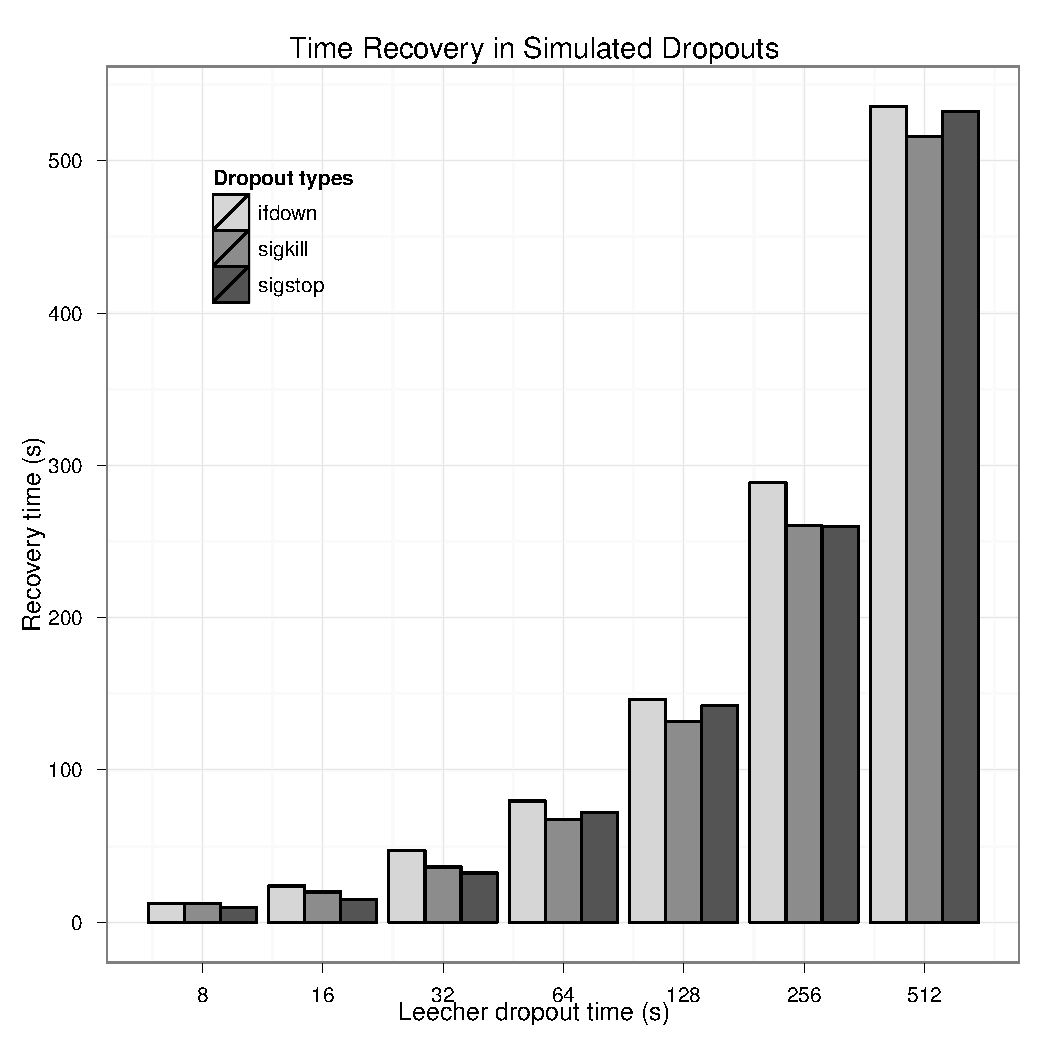
\includegraphics[width=0.5\textwidth]{src/img/virt-infra/recovery-in-simulated-dropouts.pdf}
  \end{center}
  \caption{Time Recovery with Respect to Dropout Interval}
  \label{fig:virt-infra:time-recovery}
\end{figure}

As concluding remarks, the first solution (\textbf{ifdown}) brings down the
network interface of the peer in order to simulate the end of the connection.
Results have shown that recovery time, although in the same range, is higher
than the other methods and we conclude that such a solution would be mostly
suitable for simulating connection dropouts due to network failure.

The second solution (\textbf{suspend}) suspends clients during the simulated
dropout (using SIGSTOP) and resumes them afterwards (using SIGCONT). Although
suspending peers is not a common action, results have shown that this method
is similar to the \textbf{stop} method with respect to recovery time. In an
environment where suspending peers is easier to be achieved than stopping them,
such a solution could prove suitable and provide realistic results.

The third solution (\textbf{stop}) consists of stopping (using SIGKILL) and
restarting the clients. This solution (although aggressive) is considered to
be the best approximation of a realistic behaviour of a connection dropout, as
peers have typically high dynamics when entering and exiting a swarm.

\section{Deployed Setup and Experimental Scenarios}
\label{sec:virt-infra:setup-scenarios}

The complete infrastructure, using automation, virtualization, connection
dropout simultion, allows the automatic deployment and management of a wide
variety of Peer-to-Peer scenarios. Each OpenVZ virtualized hosts runs a single
BitTorrent client (or tracker) and collects relevant information for
subsequent analysis. The commander station defines the configuration of the
new scenario and then deploys it on top of the virtualized infrastructure.
Bandwidth limitation, client types, ports to be used, churn rate, torrent
files are setup for the given scenario.

One such experiment simulates swarms comprising of a single seeder and 39
initial leechers. 19 leechers are high bandwidth peers (512KB/s download
speed, 256KB/s upload speed) and 20 leechers are low bandwidth peers (64KB/s
download speed, 32KB/s upload speed).

The total time of an experiment involving all 40 peers and a 700MB CD image
file is around 4 hours. It only takes about half an hour for the high
bandwidth clients to download it.

We have been using Linux Traffic Control (\texttt{tc}) tool combined with
iptables set-mark option to limit download and upload traffic to and from a
VE.

\subsection{Performance Evaluation Experiments}

This experimental setup used only six hardware nodes from the infrastructure.
Most of our experiments were simultaneous download sessions. Each system ran a
specific client in the same time and conditions as the other clients. Results
and logging data were collected after each client completed its download.

\subsection{Results}

\begin{table}[ht]
  \centering
  \begin{tabular}{@{}lrrrr@{}}
    \toprule
    & \textbf{Test1} & \textbf{Test2} & \textbf{Test3} &
    \textbf{Test4} \\
    \midrule
    file size & 908MB & 4.1GB & 1.09GB & 1.09GB	\\
    seeders & 2900 & 761 & 521 & 496	\\
    leechers & 2700 & 117 & 49 & 51	\\
    \midrule
    \textbf{Client} & \multicolumn{4}{c}{Download Time (seconds)} \\
    \midrule
    aria2c & 4620 & 3233 & 580 & 623 \\
    azureus & 1961 & 2313 & N/A & 420 \\
    bittorrent & 17580 & 3639 & 1560 & 840 \\
    libtorrent & \textbf{581} & \textbf{913} & \textbf{150} & \textbf{134} \\
    transmission & 2446 & 3180 & 420 & 300 \\
    tribler & 2040 & 1260 & N/A & N/A \\
    \bottomrule
  \end{tabular}
  \caption{Test Swarms Results}
  \label{table:virt-infra:testsw}
\end{table}

Table~\ref{table:virt-infra:testsw} presents a comparison of the BitTorrent
clients in four different scenarios. Each scenario means a different swarm.
Although many data were collected, only the total download time is featured in
the table.
